\newpage
\subsection{Caso d'uso UC17: Login con LinkedIn}
\label{UC17}
\begin{figure}
	\centering
	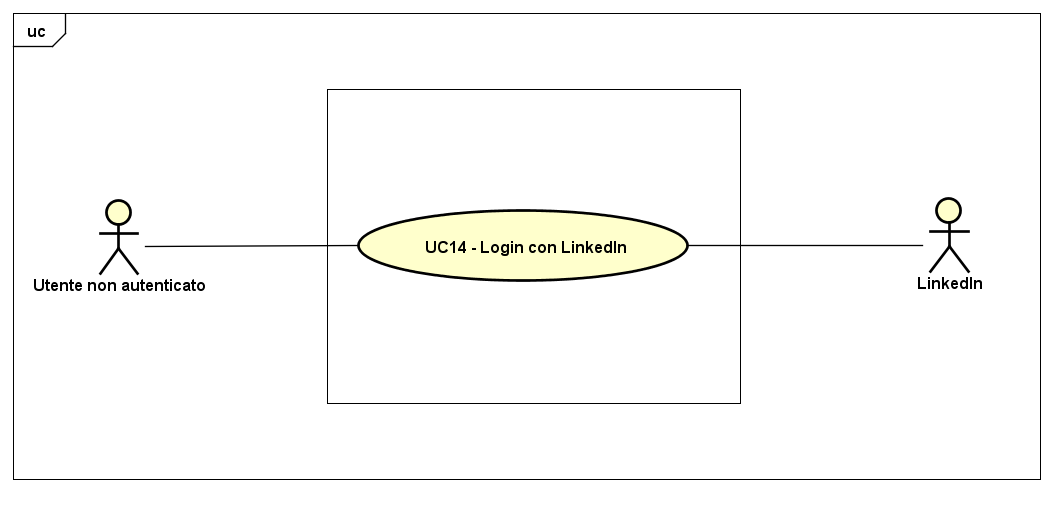
\includegraphics[scale=0.48]{UML/UC17.png}
	\caption{UC17: Login da LinkedIn}
\end{figure}
\FloatBarrier
\begin{itemize}
	\item \textbf{Attori}: utente non autenticato, LinkedIn;
	\item \textbf{Descrizione}: l'attore può autenticarsi utilizzando LinkedIn;
	\item \textbf{Precondizione}: l'attore visualizza la pagina di login e sceglie il login con LinkedIn;
	\item \textbf{Postcondizione}: l'attore è autenticato;
	\item \textbf{Scenario principale}: l'attore effettua il login tramite LinkedIn.
\end{itemize}